\chapter{Исследование фазового перехода и критического поведения в модели Поттса с числом состояний спина \texorpdfstring{$q=3$}{q=3} на гексагональной решетке методом Монте-Карло}

\subsubsection*{Ключевые слова}

Модель Поттса, фазовые переходы, критическое поведение

\subsubsection*{Реферат}

Объектом исследования является модель Поттса с числом состояний спина $q=3$ на гексагональной решетке. Целью НИР является: исследование фазового перехода и критического поведения в двумерной трехкомпонентной ($q=3$) модели Поттса на гексагональной решетке;

\paragraph*{Методы численного эксперимента:}

Метод Монте-Карло (кластерный алгоритм Вольфа).

\subsubsection*{Полученные результаты:}

С применением численных методов Монте-Карло показано, что в модели Поттса с числом состояний спина $q=3$ на гексагональной решетке наблюдается фазовый переход второго рода с критическими показателями соответствующие классу универсальности трехкомпонентной модели Поттса.

% Основная часть

\section**{Введение}

В физике конденсированных сред огромный интерес вызывают как фазовые переходы (ФП), так и связанные с ними критические явления в чистых и разбавленных спиновых системах. На разработку эффективной теории ФП и КЯ были затрачены колоссальные усилия и к настоящему моменту времени в этом направлении достигнут существенный прогресс. Создание теории Л.Д. Ландау и разработка флуктуационной теории фазовых переходов \cite{bib:bab-1}, идеи, заложенные в теории ренормализационной группы и \varepsilon-разложения \cite{bib:bab-2, bib:bab-3, bib:bab-4}, предложенные Вильсоном, а также применение гипотезы подобия (скейлинг), основы которой были заложены в 60-х годах \cite{bib:bab-1, bib:bab-5}, с последующим решением большого количества технических вопросов, позволили достичь колоссального прогресса в понимании процессов, происходящих при ФП. Кроме того, развит мощный математический аппарат, оказавшийся полезным не только для теории критических явлений, но и ряда весьма далеких от нее областей физики.

Существенный вклад в строгую количественную теорию кооперативных явлений в спиновых системах внесли также методы высоко- и низкотемпературных разложений \cite{bib:bab-6, bib:bab-7}. Было показано, что критические индексы (КИ) не зависят от величины спина, а если и зависят, то настолько слабо, что этой зависимостью даже в хорошем приближении можно пренебречь \cite{bib:bab-6}. Полученные закономерности позволили сформулировать гипотезу универсальности для статического критического поведения: критическое поведение (КП) зависит от размерности пространства (решетки), топологии параметра порядка, симметрии гамильтониана, радиуса характерного взаимодействия.

Из этой гипотезы следует, что в рамках одного класса универсальности для всех спиновых систем, испытывающих фазовый переход второго рода, критические индексы являются одинаковыми. В один и тот же класс универсальности попадают, столь непохожие на первый взгляд, системы как жидкости, магнетики, сегнетоэлектрики, сверхпроводники и другие. Следует отметить, что теоретические исследования показывают, что в двумерных моделях Поттса фазовый переход будет первого рода (со скрытой теплотой перехода), когда $q>4$ и непрерывным (без скрытой теплоты) при $q\leq4$. Результаты теоретических исследований \cite{bib:bab-8, bib:bab-9} ничего не говорят о том, каковы критические показатели при $q\leq4$. Это связано с тем, что теоретические подходы при рассмотрении модели Поттса сталкиваются с большими и труднопреодолимыми проблемами. Двумерная модель Поттса с $q=3$ и $q=4$ до настоящего времени не решена точно. Изучение магнитных и тепловых свойств в этих моделях в чистом и разбавленном (немагнитной примесью) режиме на различных двумерных решетках имеет важное фундаментальное и прикладное значение и их исследование к настоящему времени является своевременным.

\paragraph{Модель и методика.} Модель Поттса на гексагональной решетке представлена на рис.~\ref{fig:bab-1}.
\begin{figure}[ht]
    \centering
    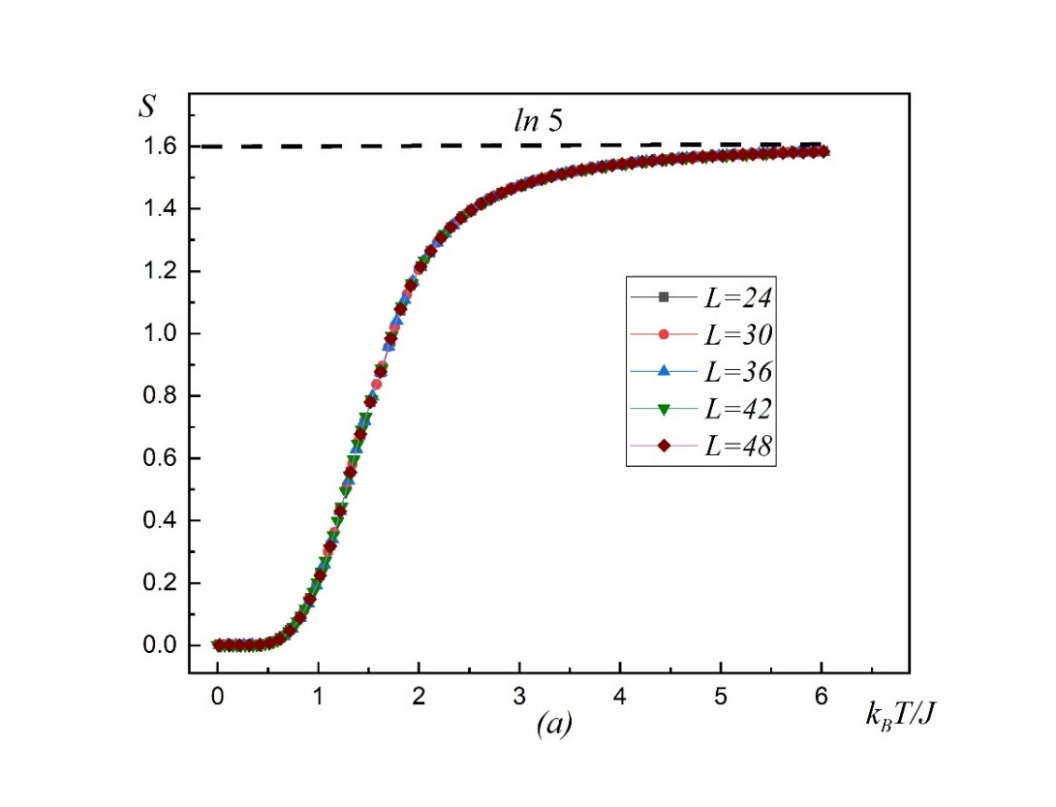
\includegraphics[trim={0 0 0 7.5cm}, clip]{bab/image1.jpeg}
    \caption{Трехкомпонентная модель Поттса на гексагональной решетке.}
    \label{fig:bab-1}
\end{figure}

Гамильтониан ферромагнитной модели Поттса c числом состояний спина $q=3$ может быть представлен в следующем виде \cite{bib:bab-8, bib:bab-9}:
\begin{equation}
    \label{eq:bab-1}
    H = -\frac{1}{2} J \sum_{i, j} \delta(S_i, S_j), \quad S_i = P_1, P_2, P_3
\end{equation}
где $J$ -- параметр ферромагнитного ($J>0$) взаимодействия ближайших спинов, $P_i$ число состояний выбранного спина $S_i$. Из аналитических теорий известно, что в двумерных моделях Поттса с числом состояний спина $q=3$ и $q=4$ в однородном состоянии наблюдается ФП второго рода. К настоящему времени критическое поведение этих моделей на различных решетках не изучено достаточно хорошо.

Все исследования, проведены с использованием высокоэффективного кластерного алгоритма Вольфа \cite{bib:bab-10} метода Монте-Карло (МК). Расчеты проводились для систем с периодическими граничными условиями. Исследовались системы с линейными размерами $L=10 - 320$. Для вывода системы в равновесное состояние вычислялось время релаксации $\tau_0$ соответствующее для каждой системы с линейными размерами $L$. Этот неравновесный участок отбрасывали. Кроме того, усреднение проводилось по участку марковской цепи длиной $\tau=400\tau_0$. Причем, для самой большой системы $L=320$, $\tau_0 = 2 \times 10^4$ МК шагов/спин.

\section*{Результаты}

Наблюдение за температурным ходом энергии $U$, намагниченности $m$, теплоемкости $C$ и восприимчивости $\chi$ осуществлялось с использованием следующих выражений \cite{bib:bab-9, bib:bab-11}:
\begin{gather}
    \label{eq:bab-2}
    U = \left[\left<U\right>\right]=\frac1N\left[\left<H\right>\right], \\
    \label{eq:bab-3}
    m = \frac{\left[q\left(\frac{N_{\max}}{N}\right) - 1\right]}{q - 1}, \\
    \label{eq:bab-4}
    C = \left(NK^2\right)\left(\left<m^2\right>-\left<m\right>^2\right), \\
    \label{eq:bab-5}
    \chi = (NK) \left(\left<m^2\right>-\left<m\right>^2\right),
\end{gather}
где $K = \left|J\right| / k_B T$, $N_{\max} = \max \left\{N_1, N_2, N_3\right\}$, $N_i$ -- число спинов в состоянии с $q=P_i$, $N$ -- число узлов решетки, угловые скобки означают термодинамическое усреднение.
\begin{figure}[ht]
    \begin{minipage}[c]{0.45\linewidth}
        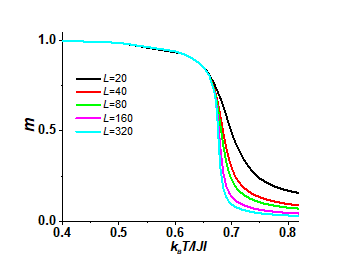
\includegraphics[width=\linewidth]{bab/image12.png}
        \caption{Температурная зависимость намагниченности $m$ для модели Поттса с $q=3$ на гексагональной решетке.}
        \label{fig:bab-2}
    \end{minipage}
    \hfill
    \begin{minipage}[c]{0.45\linewidth}
        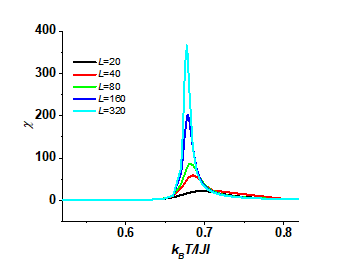
\includegraphics[width=\linewidth]{bab/image11.png}
        \caption{Температурная зависимость восприимчивости $\chi$ для модели Поттса с $q=3$ на гексагональной решетке.}
        \label{fig:bab-3}
    \end{minipage}
\end{figure}

На рисунках \ref{fig:bab-2} и \ref{fig:bab-3} представлены характерные зависимости намагниченности $m$ и 
восприимчивости $\chi$ для трехкомпонентной модели Поттса на гексагональной решетке от температуры соответственно. Здесь и далее на всех рисунках погрешность данных не превышает размеров символов, используемых для построения графиков. Как видно из этих рисунков, для всех рассмотренных систем наблюдается поведение характерное для фазового перехода второго рода.

В численных методах для определения температуры и рода ФП хорошо зарекомендовал метод кумулянтов Биндера четвертого порядка \cite{bib:bab-12}
\begin{gather}
    \label{eq:bab-6}
    V_L(T) = 1 - \frac{\left<E^4(T; L)\right>_L}{3\left<E^2(T; L)\right>_L^2}, \\
    \label{eq:bab-7}
    U_L(T) = 1 - \frac{\left<m^4\right>_L}{3\left<m^2\right>_{L^2}},
\end{gather}
где $E$ и $m$ -- энергия и намагниченность рассматриваемой системы с линейным размером $L$. Выражения \eqref{eq:bab-6} и \eqref{eq:bab-7} позволяют определить температуру $T_l$ фазового перехода с большой точностью в ФП первого и второго рода соответственно. Как известно ФП второго рода характеризуются следующими отличительными особенностями \cite{bib:bab-13}: усредненная величина $V_L(T)$ стремится к тривиальному значению $V^*$ согласно выражению
\begin{equation}
    \label{eq:bab-8}
    V(T) = V^* + bL^{-d}
\end{equation}
при $L \to \infty$ и $T=T_c(L)$, где $V^* = 2/3$, а кумулянты Биндера $U_L(T)$ в критической области имеют четко выраженную точку пересечения. Указанные особенности для кумулянтов Биндера четвертого порядка $V_L(T)$ и $U_L(T)$ продемонстрированы на рис.~\ref{fig:bab-4} и \ref{fig:bab-5} соответственно для ферромагнитной трехкомпонентной модели Поттса на гексагональной решетке. Методика определения рода фазового перехода этим методом подробно описана в работе \cite{bib:bab-14}. Как видно из рис.~\ref{fig:bab-4} температура ФП в трехкомпонентной модели Поттса на гексагональной решетке $T_c=0.673(2)$. Следует отметить, что для двумерных моделей Поттса с числом состояний спина $q$ из соображений дуальности квадратной, треугольной и гексагональной решетки были получены простые полиномиальные выражения, позволяющие определить критическую температуру (см. \cite{bib:bab-8}). Однако эти выражения справедливы только для моделей Поттса с $q>3$ и $q=2$ \cite{bib:bab-9}.
\begin{figure}[ht]
    \begin{minipage}[c]{0.45\linewidth}
        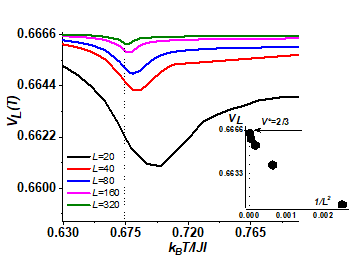
\includegraphics[width=\linewidth]{bab/image18.png}
        \caption{Температурная зависимость кумулянтов Биндера $V_L(T)$ для трехкомпонентной модели Поттса на гексагональной решетке.}
        \label{fig:bab-4}
    \end{minipage}
    \hfill
    \begin{minipage}[c]{0.45\linewidth}
        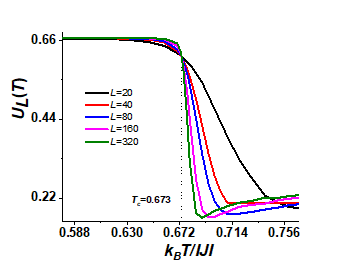
\includegraphics[width=\linewidth]{bab/image17.png}
        \caption{Температурная зависимость кумулянтов Биндера $U_L(T)$ для трехкомпонентной модели Поттса на гексагональной решетке.}
        \label{fig:bab-5}
    \end{minipage}
\end{figure}

Для рассмотренной модели Поттса на гексагональной решетке нами исследовалось критическое поведение на основе применения теории конечно-размерного скейлинга (КРС). Из соотношений этой теории следует, что для достаточно большой системы с ПГУ при температуре $T=T_c$ намагниченность $m$, восприимчивость $\chi$ удовлетворяют следующим аналитическим выражениям \cite{bib:bab-15}
\begin{gather}
    \label{eq:bab-9}
    m \sim L^{-\beta / v}, \\
    \label{eq:bab-10}
    \chi \sim L^{\gamma / v}.
\end{gather}

Эти соотношения были нами использованы для определения $\beta / v$ и $\gamma / v$. Для аппроксимации температурной зависимости теплоемкости от $L$ использовалось выражение
\begin{equation}
    \label{eq:bab-11}
    C = A + BL^{\alpha / v},
\end{equation}
где $A$, $B$ -- некоторые коэффициенты.

В соответствии с теорией КРС в точке ФП для критического индекса радиуса корреляции $v$ выполняется соотношение \cite{bib:bab-16}
\begin{equation}
    \label{eq:bab-12}
    v_n = L^{\frac{1}{v}} g_{v_n},
\end{equation}
где $g_{v_n}$ -- некоторая постоянная, а в качестве $V_n$ могут выступать:
\begin{equation}
    \label{eq:bab-13}
    V_i = \frac{\left<m^i E\right>}{\left<m^i\right>} - \left<E\right>, \quad (i = 1, 2, 3).
\end{equation}

Для расчета критических индексов (КИ) $\beta$, $\gamma$, $\alpha$, и $v$ строились зависимости $m$, $\chi$, $C$, и $V_n$ от $L$ (см. рис.~\ref{fig:bab-6}). Анализ данных, выполненный с использованием нелинейного метода наименьших квадратов, позволил определить значения $\beta / v$, $\gamma / v$, $\alpha / v$ и $1/v$ (см. Таблицу~\ref{tab:bab-1}). Затем, используя значения $v$, полученное в рамках данного исследования, определялись все остальные индексы $\beta$, $\gamma$, и $\alpha$. Точность критических индексов согласно выражениям теории КРС \eqref{eq:bab-9}-\eqref{eq:bab-12} в большей степени зависит от правильности учета данных для разных линейных размеров $L$. В наших расчетах строго контролировались данные для всех рассмотренных систем и при их незначительном отклонении от аппроксимирующей прямой процедура фитирования проводилась заново с отсеканием данных для $L<L_{\min}$. Такой отбор данных для разных линейных размеров $L$ позволяет заметно уменьшить погрешность в значениях КИ.
\begin{table}[ht]
    \centering
    \caption{Критические индексы для трехкомпонентной модели Поттса на гексагональной решетке}
    \label{tab:bab-1}
    \scriptsize
    \begin{tabular}{|p{2cm}*{9}{|c}|}
        \hline
        метод & $v$ & $1/v$ & $\alpha$ & $\alpha/v$ & $\gamma$ & $\gamma/v$ & $\beta$ & $\beta/v$ & $\alpha + 2\beta + \gamma = 2$ \\
        \hline
        Теория, \cite{bib:bab-9} & \makecell{5/6 \\ 0.83} & \makecell{6/5 \\ 1.20} & \makecell{1/3 \\ 0.333} & \makecell{2/5 \\ 0.40} & \makecell{13/9 \\ 1.444} & \makecell{26/15 \\ 1.733} & \makecell{1/9 \\ 0.111} & \makecell{2/15 \\ 0.133} & 2.0 \\
        \hline
        МК, гексагональная решетка (наши данные) & 0.847(3) & 1.180(2) & 0.327(3) & 0.387(3) & 1.446(1) & 1.708(3) & 0.107(3) & 0.127(3) & 1.99 \\
        \hline
        МК \cite{bib:bab-17}, квадратная решетка & & & & 0.46(8) & & 1.736(1) & & 0.131(1) & \\
        \hline
    \end{tabular}
    \medskip
\end{table}
\begin{figure}[ht]
    \begin{subfigure}{0.5\textwidth}
        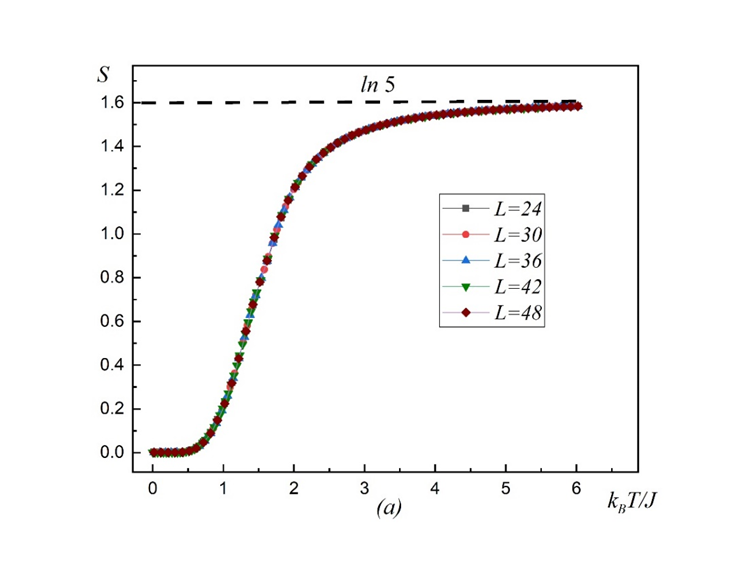
\includegraphics[width=0.9\linewidth]{bab/image24.png}
    \end{subfigure}
    \begin{subfigure}{0.5\textwidth}
        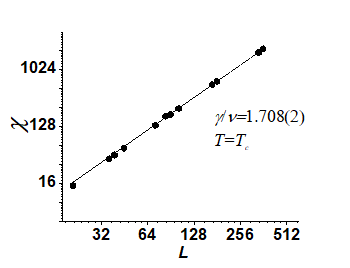
\includegraphics[width=0.9\linewidth]{bab/image25.png}
    \end{subfigure}
    \begin{subfigure}{0.5\textwidth}
        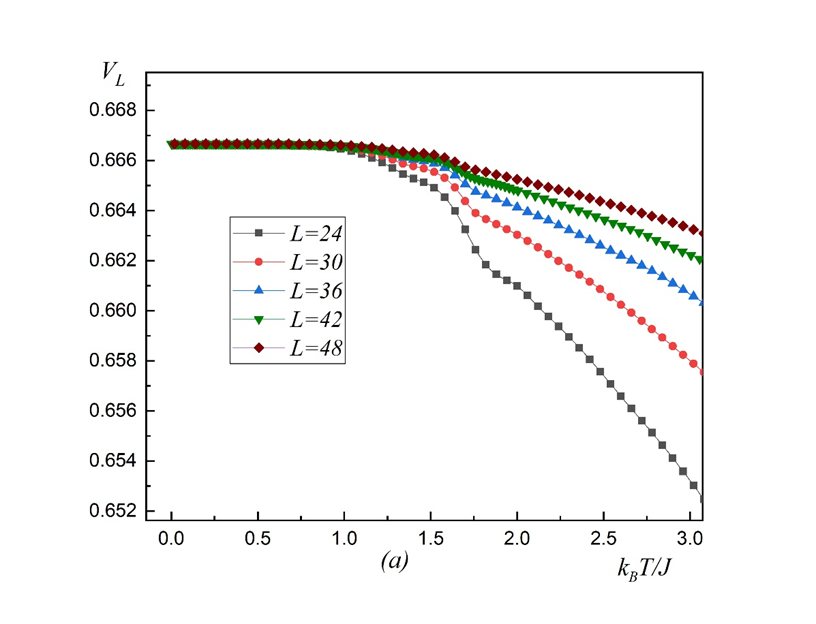
\includegraphics[width=0.9\linewidth]{bab/image27.png}
    \end{subfigure}
    \begin{subfigure}{0.5\textwidth}
        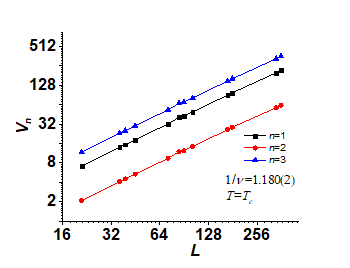
\includegraphics[width=0.9\linewidth]{bab/image26.png}
    \end{subfigure}
    \caption{Зависимость намагниченности $m$, восприимчивости $\chi$, теплоемкости $C$, для трехкомпонентной модели Поттса на гексагональной решетке от линейных размеров системы $L$ при $T = T_c$.}
    \label{fig:bab-6}
\end{figure}

\section*{Заключение}

Таким образом, полученные данные в результате компьютерного моделирования трехкомпонентной модели Поттса на гексагональной решетке свидетельствуют, что в ней наблюдается фазовый переход второго рода. При этом:
\begin{enumerate}
    \item Критическое поведение не демонстрирует мультипликативные логарифмические поправки к намагниченности, восприимчивости и теплоемкости, которые ранее были выявлены для модели Поттса с $q=4$ на квадратной решетке (см. работы, \cite{bib:bab-17,bib:bab-18}).
    \item Конечномерный анализ полученных данных демонстрирует наличие фазового перехода второго рода с критическими показателями (см. Табл.~\ref{tab:bab-1}), соответствующими классу универсальности модели Поттса с $q=3$ на квадратной решетке \cite{bib:bab-17}.
\end{enumerate}

\section*{Публикации}

\textbf{В центральных Российских изданиях:}
\begin{enumerate}
    \item Бабаев А.Б., Муртазаев А.К. Моделирование трехкомпонентной модели Поттса на гексагональной решетке методом Монте-Карло // Физика металлов и металловедение. -- 2023. -- Т.124. -- \textnumero 7. -- С. 577--583. \\ \url{https://www.sciencejournals.ru/view-article/?j=fizmet\&y=2023\&v=124\&n=7\&a=FizMet2360045Babaev}
\end{enumerate}

\textbf{В трудах международных и российских конференций:}
\begin{enumerate}
    \item Бабаев А.Б., Муртазаев А.К., Абуев Я.К., Ибаев Д.Г., Бабаев М.А. Исследование критического поведения трехкомпонентной модели Поттса на гексагональной решетке методом Монте-Карло // Сборник трудов международной конференции, посвященной 300-летию Российской академии наук -- 10-15 сентября 2023 г., Махачкала, С. 63--56.
\end{enumerate}

% NOTE: was in appendix
% \appendix

\section*{ПРАКТИЧЕСКОЕ ПРИМЕНЕНИЕ \\ АПРОБАЦИЯ ПОЛУЧЕННЫХ РЕЗУЛЬТАТОВ}

\textbf{Полученные нами результаты были представлены на следующих конференциях:}

Международная конференция, посвященная 300-летию Российской академии наук, 10-15 сентября 2023 г., Махачкала:
\begin{enumerate}
    \item Бабаев А.Б., Муртазаев А.К., Абуев Я.К., Ибаев Д.Г., Бабаев М.А. Исследование критического поведения трехкомпонентной модели Поттса на гексагональной решетке методом Монте-Карло (стендовый доклад Бабаева А.Б.)
\end{enumerate} 